\documentclass{scu-thesis}
\usepackage{amsmath}	% for advanced typesetting of mathematics
\usepackage{graphicx}	% for including graphics
\usepackage{natbib}	    % for better citation styles
\usepackage{txfonts}	% for using the Times-Roman font
\usepackage{booktabs}   % for table styling
\usepackage{makecell}   % for multiple line table cells
\usepackage{multirow}   % for multiple row table cells

% These must be set first ... the rest of the thesis commands rely on them.

\author{Jake Day}
\author{Yutong Li}
\author{Sam Rietz}
\author{Brendan Watamura}
\title{H.E.A.R.T.}
\department{Department of Computer Engineering}
\degree{Bachelor of Science in Computer Science and Engineering}

% Only bachelor's theses should have multiple authors and/or be from
% multiple departments.  Signatures required:
%
% Bachelor's theses: advisor(s), department chair(s)
% Master's theses: advisor, reader, department chair
% Doctoral theses: doctoral committee (including advisor), department chair

\begin{document}
\frontmatter
\signature{Thesis Advisor}
\signature{Thesis Advisor}
\signature{Department Chair}
\signature{Department Chair}

\maketitle
\begin{abstract}
A good abstract is a concise summary (1--2 paragraphs) of the entire
project: introduction, problem statement, work accomplished, results,
conclusions, and recommendations. When you write the abstract, imagine
that the reader will not read anything else, but that you must get
your major point across immediately. This requires efficiency of words
and phrases. An abstract is written to stand alone, without jargon or
reference to figures and tables in the report body.
\end{abstract}


\tableofcontents
\listoffigures
\listoftables

\mainmatter
\chapter{Introduction} % Jake

\section{Motivation}


Parents, specifically those of at-risk youth, are not providing their children with responsive caregiving. 
These children are growing up in an environment in which their parents have low emotional resilience, a quality developed early on in one's childhood. 
When parents display this behavior in front of their children, these children grow up susceptible to stress and emotional distress, perpetuating a vicious cycle. 
Healthy parenting and family resilience in early childhood has been shown to be an important factor in effectively managing stress, promoting school readiness and achievement, and preventing adolescents from participating in high-risk behaviors.

At this time, there lacks a means to teach emotional resilience to reach a wide target audience. 
Traditional solutions such as psychotherapy or medication prescribed by a doctor may ameliorate the symptoms of stress, but fail to address the underlying issue. 
Even with the emergence of electronic wearable devices (i.e. stress detectors), this solution alone fails to help as they simply alert individuals if they are stressed, potentially worsening symptoms with constant reminders. 
Dr. Barbara Burns, professor and director of child studies at Santa Clara University, presents the most promising solution at this time; her Resilient Families Program (RFP) aims to promote family and community resilience with community-led, science-based parent education programs.
However, the program's outreach is severely limited to the number of individuals Dr. Burns can train at a given time. 

A former senior design project collaborated with Dr. Burns and came up with a VR Empathy Training Tool. 
The user can interact with a crying child and therefore learn how to handle stress (under certain circumstances). 
However, the project has the same level of difficulty for all individuals regardless of the difference of their emotional resilience. 
The project also lacks a sense of immersion and virtual "presence", which is a key component in creating empathy within VR. 
Furthermore, their design decision to measure stress using only heart rate is non-comprehensive.

Fortunately, resilience is not a fixed characteristic; it can be learned. 
As individuals, we can build an awareness of the situations in which we are least resilient and focus our efforts on developing personal resilience there. 

\section{Solution}

Our solution builds upon the framework laid out by RFP. We propose a virtual reality (VR) mobile application that allows parents to interact with a virtual child. 
The child will display signs of distress and will react based upon the user's decision. 
Based on prior research, we also believe allowing parents to take the perspective of the child will expedite their development toward empathy. 
Unlike prior solutions, ours does more than inform users they are stressed. 
The intensity of the experience will vary based on perceived stress levels.
This teaches users how to handle stress in a productive manner without overwhelming them from the start.
To address the lack of outreach of RFP, our solution will utilize an accessible and low cost VR implementation.
Our solution will also provide users with the ability to track their progress, based on stress levels exhibited during each session.
As a result, different individuals can get personalized training.

\chapter{Requirements} % Jake [DONE]

\section{Functional Requirements}
    \subsection{Critical}
        \begin{itemize}
            \item The system will function on iOS devices using Google Cardboard.
            \item The system will inform the user right after it detects that the user is stressed.
            \item The system will train users in emotional resilience.
            \item 	The system will keep track of users' personal progress.
            \item The system will collect user data anonymously (including personal progress).
            \item The system will measure user heart rate using the phone's camera lens.
            \item The system will adjust difficulty of the game, based on how well the individual handles stress and his/her stress level.
\end{itemize}
    \subsection{Recommended}
        \begin{itemize}
            \item The VR experience will contain spatialized audio.
            \item The VR experience will halt if the user is too uncomfortable. 
            \item Users' data will be sent for research, with their consent.
        \end{itemize}
    \subsection{Suggested}
        \begin{itemize}
            \item The system will function on Android devices.
        \end{itemize}
\section{Non-Functional Requirements}
    \subsection{Critical}
        \begin{itemize}
            \item The application will be user-friendly.
            \item The VR experience will be immersive.
            \item The VR experience will be a maximum of 2 minutes long.
            \item The system will be able to change the difficulty of the game in real time based on the user's performance.
        \end{itemize}
    \subsection{Recommended}
        \begin{itemize}
            \item The system will be supportive of multiple languages.
            \item The application will be energy efficient.
        \end{itemize}
    \subsection{Suggested}
        \begin{itemize}
            \item The system will be maintainable and portable.
        \end{itemize}
\section{Design Constraints}
\begin{itemize}
\item 	Compliance to applicable laws, regulations and standards
\item 	Style guide
\item 	Sensory Design
\item 	Usability principles, frameworks and standards
\item 	Design principle
\item 	Integration
\end{itemize}
     
     
\chapter{Use Cases} % Yutong / Jake [DONE]

The two actors involved are users and developers. Each of their respective functions are listed in Figure~\ref{fig:use-cases}.

\section{User Use Cases}
The users can play the game from both their own perspective, which will be interacting with a virtual child, and the child's perspective. The users can also keep track of their personal progress by checking out the report generated.

\begin{table}[h!]
\centering
\caption{Play as Parent Use Case}
\label{table:game-with-child}
\vspace{5mm}
\resizebox{0.66\textwidth}{!}{%
\begin{tabular}{@{}l|lllll@{}}
\toprule
\textbf{Use Case Name}      & Play as parent \\
\midrule
\textbf{Goal}               & Interact with virtual child \\ 
\midrule
\textbf{Actor(s)}           & User \\
\midrule
\textbf{Precondition(s)}    & Be logged in as User \\
\midrule
\textbf{Postcondition(s)}   & VR child is happy \\
\midrule
\textbf{Exception(s)}       & N/A \\
\midrule
\end{tabular}%
}
\end{table}

\begin{table}[h!]
\centering
\caption{Play as Child Use Case}
\label{table:game-with-child}
\vspace{5mm}
\resizebox{0.66\textwidth}{!}{%
\begin{tabular}{@{}l|lllll@{}}
\toprule
\textbf{Use Case Name}      & Play as child \\
\midrule
\textbf{Goal}               & Empathize with child\\ 
\midrule
\textbf{Actor(s)}           & User \\
\midrule
\textbf{Precondition(s)}    & Be logged in as User \\
\midrule
\textbf{Postcondition(s)}   & Experienced child's perspective \\ 
\midrule
\textbf{Exception(s)}       & N/A \\
\midrule
\end{tabular}%
}
\end{table}

\begin{table}[h!]
\centering
\caption{Track Personal Progress Use Case}
\label{table:game-with-child}
\vspace{5mm}
\resizebox{0.66\textwidth}{!}{%
\begin{tabular}{@{}l|lllll@{}}
\toprule
\textbf{Use Case Name}      & Track personal progress \\
\midrule
\textbf{Goal}               & View and learn from progress\\ 
\midrule
\textbf{Actor(s)}           & User \\
\midrule
\textbf{Precondition(s)}    & Be logged in as User \\
\midrule
\textbf{Postcondition(s)}   & Display historical data\\
\midrule
\textbf{Exception(s)}       & N/A \\
\midrule
\end{tabular}%
}
\end{table}

\clearpage

\section{Developer Use Cases}

With the system, the developers are able to develop personalize "training plan" based on the user data, while the users can play game and keep track of their personal progress. The developers can decide the stress level for the user by analyzing the collected user data. While measuring the current stress level of the user, the developers can adjust then the difficulty of the game based on the user's stress level in real time.


\begin{table}[h!]
\centering
\caption{Collect User Data Use Case}
\label{table:game-with-child}
\vspace{5mm}
\resizebox{0.66\textwidth}{!}{%
\begin{tabular}{@{}l|lllll@{}}
\toprule
\textbf{Use Case Name}      & Collect user data \\
\midrule
\textbf{Goal}               & Track user progress\\ 
\midrule
\textbf{Actor(s)}           & Developer \\
\midrule
\textbf{Precondition(s)}    & Be logged in as Developer \\
\midrule
\textbf{Postcondition(s)}   & User data sent to be analyzed \\
\midrule
\textbf{Exception(s)}       & N/A \\
\midrule
\end{tabular}%
}
\end{table}

\begin{table}[h!]
\centering
\caption{Analyze User Data Use Case}
\label{table:game-with-child}
\vspace{5mm}
\resizebox{0.66\textwidth}{!}{%
\begin{tabular}{@{}l|lllll@{}}
\toprule
\textbf{Use Case Name}      & Analyze user data \\
\midrule
\textbf{Goal}               & Study user progress\\ 
\midrule
\textbf{Actor(s)}           & Developer \\
\midrule
\textbf{Precondition(s)}    & Be logged in as Developer \\
\midrule
\textbf{Postcondition(s)}   & Analysis stored in centralized location \\
\midrule
\textbf{Exception(s)}       & N/A \\
\midrule
\end{tabular}%
}
\end{table}

\begin{table}[h!]
\centering
\caption{Decide Stress Level Use Case}
\label{table:game-with-child}
\vspace{5mm}
\resizebox{0.66\textwidth}{!}{%
\begin{tabular}{@{}l|lllll@{}}
\toprule
\textbf{Use Case Name}      & Decide stress level \\
\midrule
\textbf{Goal}               & Adjust game intensity\\ 
\midrule
\textbf{Actor(s)}           & Developer \\
\midrule
\textbf{Precondition(s)}    & Be logged in as Developer \\
\midrule
\textbf{Postcondition(s)}   & Stress levels calculated \\
\midrule
\textbf{Exception(s)}       & N/A \\
\midrule
\end{tabular}%
}
\end{table}

\begin{table}[h!]
\centering
\caption{Measure Current Stress level Use Case}
\label{table:game-with-child}
\vspace{5mm}
\resizebox{0.66\textwidth}{!}{%
\begin{tabular}{@{}l|lllll@{}}
\toprule
\textbf{Use Case Name}      & Measure current stress level \\
\midrule
\textbf{Goal}               & Track historical stress data\\ 
\midrule
\textbf{Actor(s)}           & Developer \\
\midrule
\textbf{Precondition(s)}    & Be logged in as Developer \\
\midrule
\textbf{Postcondition(s)}   & Heart rate readings stored in centralized location \\
\midrule
\textbf{Exception(s)}       & N/A \\
\midrule
\end{tabular}%
}
\end{table}

\begin{table}[h!]
\centering
\caption{Adjust Game Difficulty Use Case}
\label{table:game-with-child}
\vspace{5mm}
\resizebox{0.66\textwidth}{!}{%
\begin{tabular}{@{}l|lllll@{}}
\toprule
\textbf{Use Case Name}      & Adjust game difficulty \\
\midrule
\textbf{Goal}               & Personalize user experience\\ 
\midrule
\textbf{Actor(s)}           & Developer \\
\midrule
\textbf{Precondition(s)}    & Be logged in as Developer \\
\midrule
\textbf{Postcondition(s)}   & Difficulty reflects user stress\\
\midrule
\textbf{Exception(s)}       & N/A \\
\midrule
\end{tabular}%
}
\end{table}

\begin{table}[h!]
\centering
\caption{Generate Report Use Case}
\label{table:game-with-child}
\vspace{5mm}
\resizebox{0.66\textwidth}{!}{%
\begin{tabular}{@{}l|lllll@{}}
\toprule
\textbf{Use Case Name}      & Generate report \\
\midrule
\textbf{Goal}               & Record user progress\\ 
\midrule
\textbf{Actor(s)}           & Developer \\
\midrule
\textbf{Precondition(s)}    & Be logged in as Developer \\
\midrule
\textbf{Postcondition(s)}   & Report is sent to user \\
\midrule
\textbf{Exception(s)}       & N/A \\
\midrule
\end{tabular}%
}
\end{table}

\begin{figure}[ht]
    \centering
    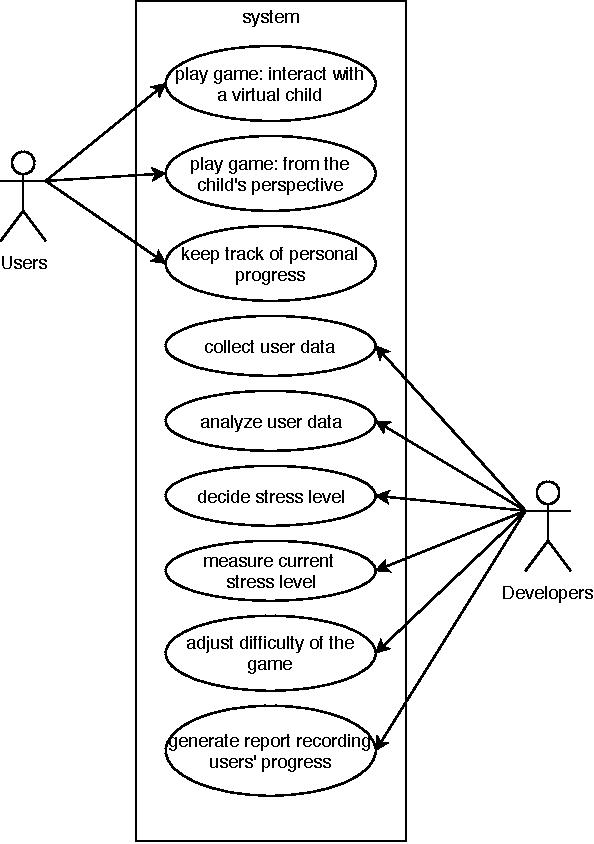
\includegraphics[width=0.66\linewidth]{use-cases}
    \caption{Use Cases}
    \label{fig:use-cases}
\end{figure}





\chapter{Activity Diagram} % Yutong

The activity diagrams shown in Figures~\ref{fig:act-div-usr} and \ref{fig:act-div-dev} describe the flow of actions when users and developers, respectively, access the application. The potential actions are based on the use cases described in Figure~\ref{fig:use-cases}.

Figure 4.1 is what the users can do with the system.
Through the system, the users can play the game as well as keep track of their progress. The users can choose to interact with a virtual child from their own perspective or interact with an adult from a child's perspective. 


Figure 4.2 is what the developers can do with the system.
Through the system, the developers can analyze collected user data and keep track of users' progress. With data analysis, the developers can detect "initial" stress, decide stress level, and measure current stress level for the users. By comparing the users' current stress level with the standard of their stress level, the developers can then personalize "training plan" for different users. 


\begin{figure}[!ht]
    \centering
    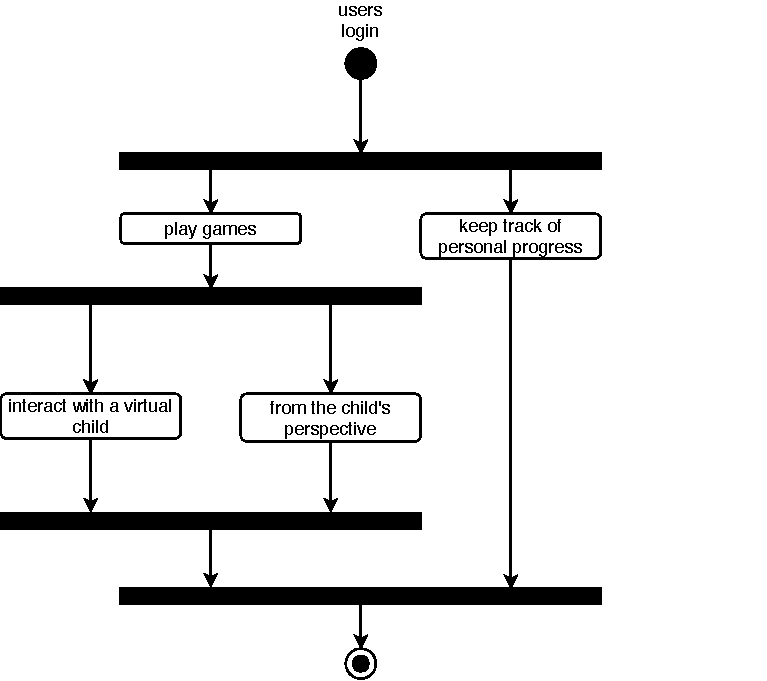
\includegraphics[width=0.75\linewidth]{activity-diagram-users}
    \caption{Users Activity Diagram}
    \label{fig:act-div-usr}
\end{figure}

\begin{figure}[!ht]
    \centering
    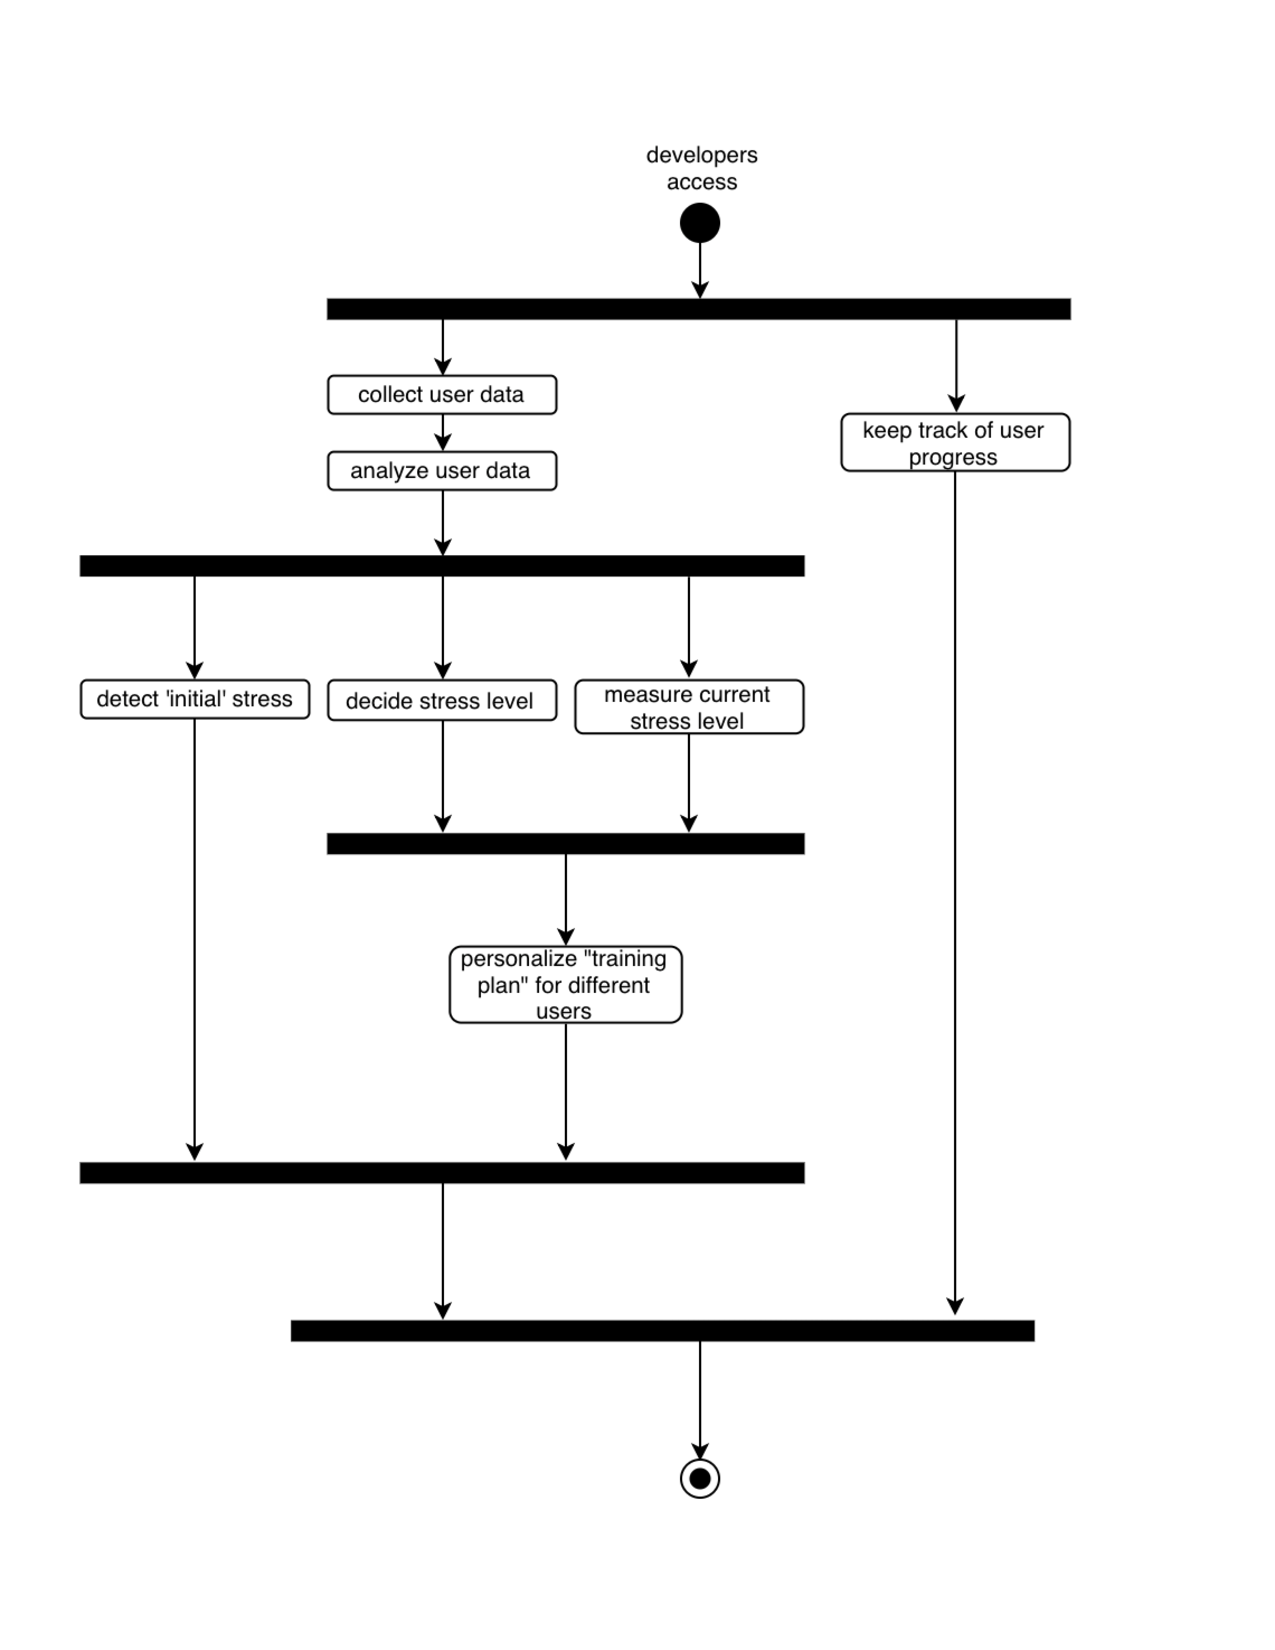
\includegraphics[width=\linewidth]{activity-diagram-developers}
    \caption{Developers Activity Diagram}
    \label{fig:act-div-dev}
\end{figure}
\chapter{Conceptual Model}

Figure~\ref{fig:con-model} shows an example of the main page for user interface. This page shows what the interaction page should look like when the user is playing the game. There are three options provided for the users that they can click on. The baby will react differently to different options.

\begin{figure}[H]
    \centering
    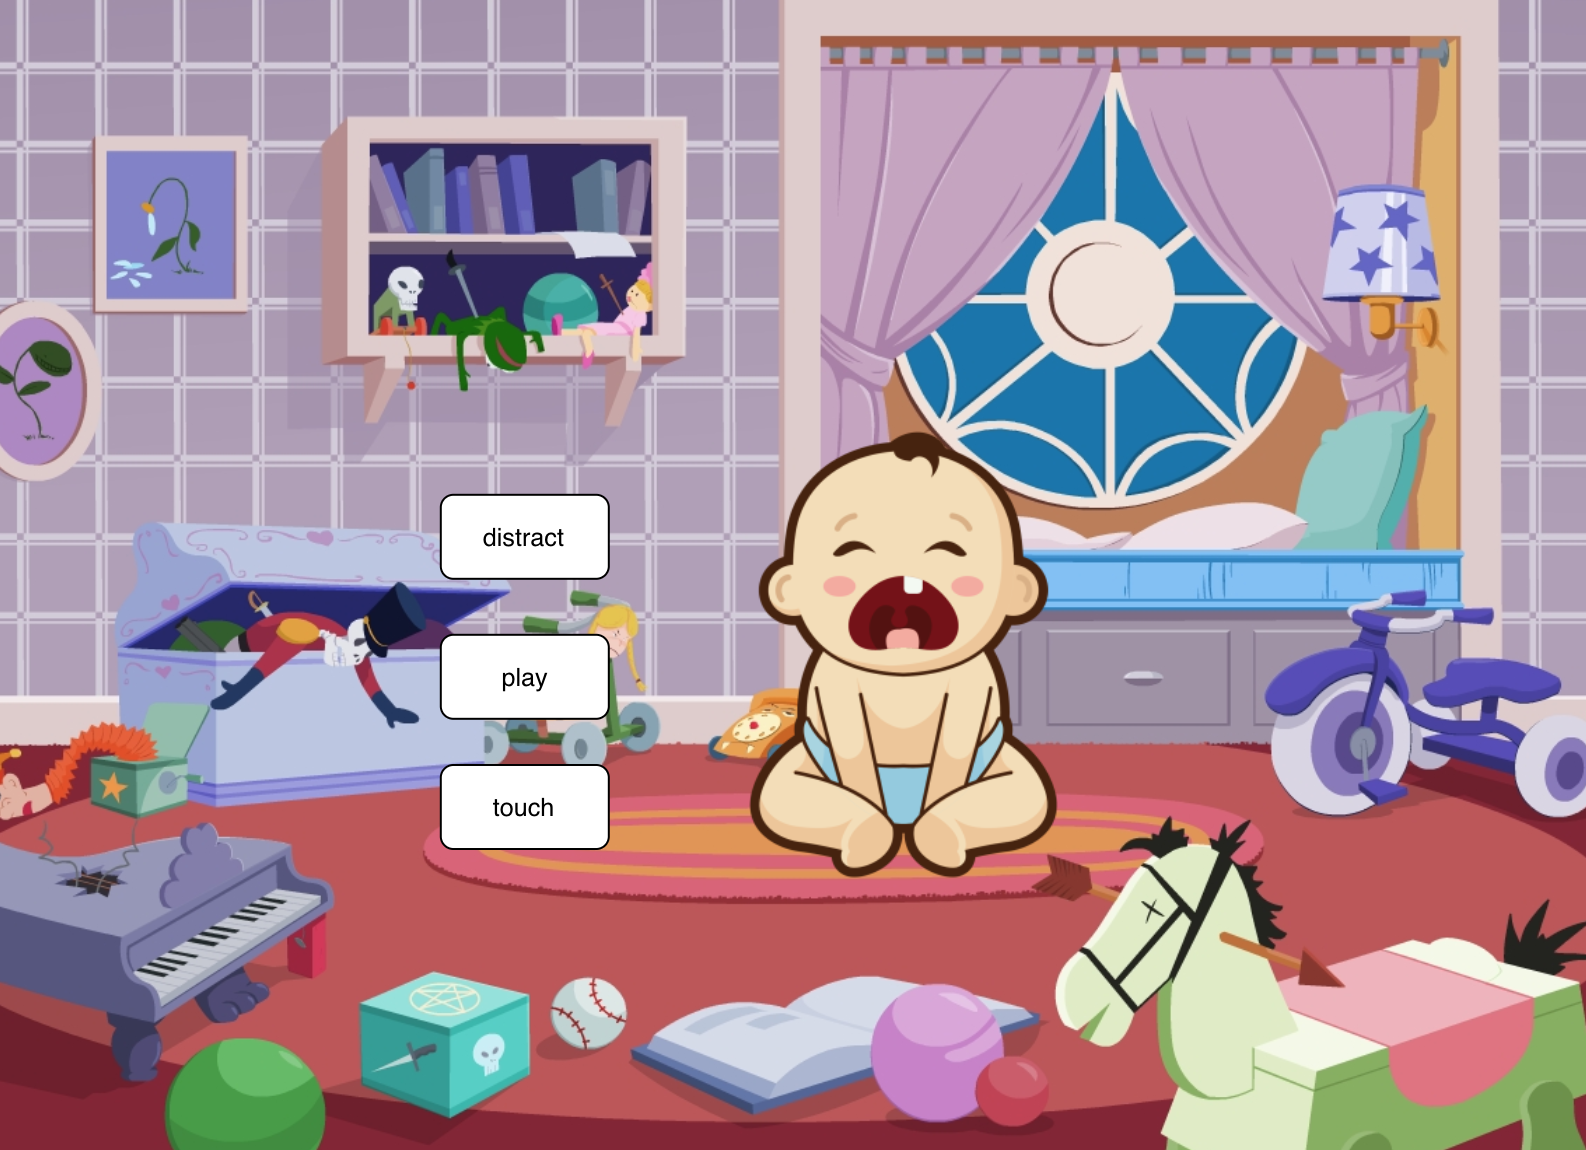
\includegraphics[width=0.75\linewidth]{conceptual-model.png}
    \caption{Conceptual Model}
    \label{fig:con-model}
\end{figure}
The users can access both the report on a single practice, and the general progress report which shows all of their practice. 

Figure~\ref{fig:report} is an example of the report that the user can view. In the report on a specific practice, the users can see the time they first got stressed and the level of stress they experienced. 

\begin{figure}[H]
    \centering
    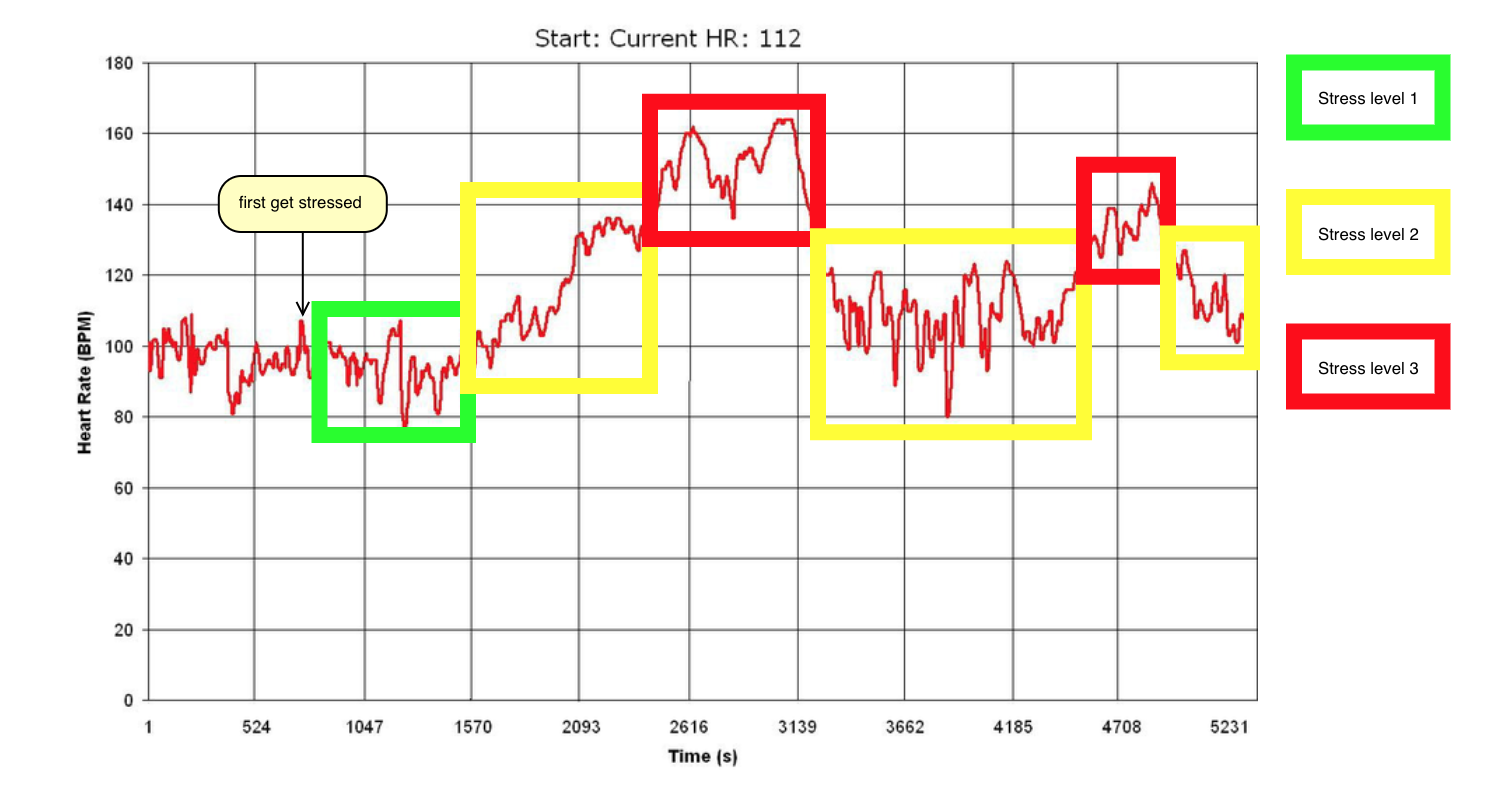
\includegraphics[width=0.75\linewidth]{heartrate.png}
    \caption{Report}
    \label{fig:report}
\end{figure}

Figure~\ref{fig:prog-rep} is an example of the progress report that the user can view. In the progress report, the users can compare their performance in different practices and check their progress under the same difficulty level.

\begin{figure}[H]
    \centering
    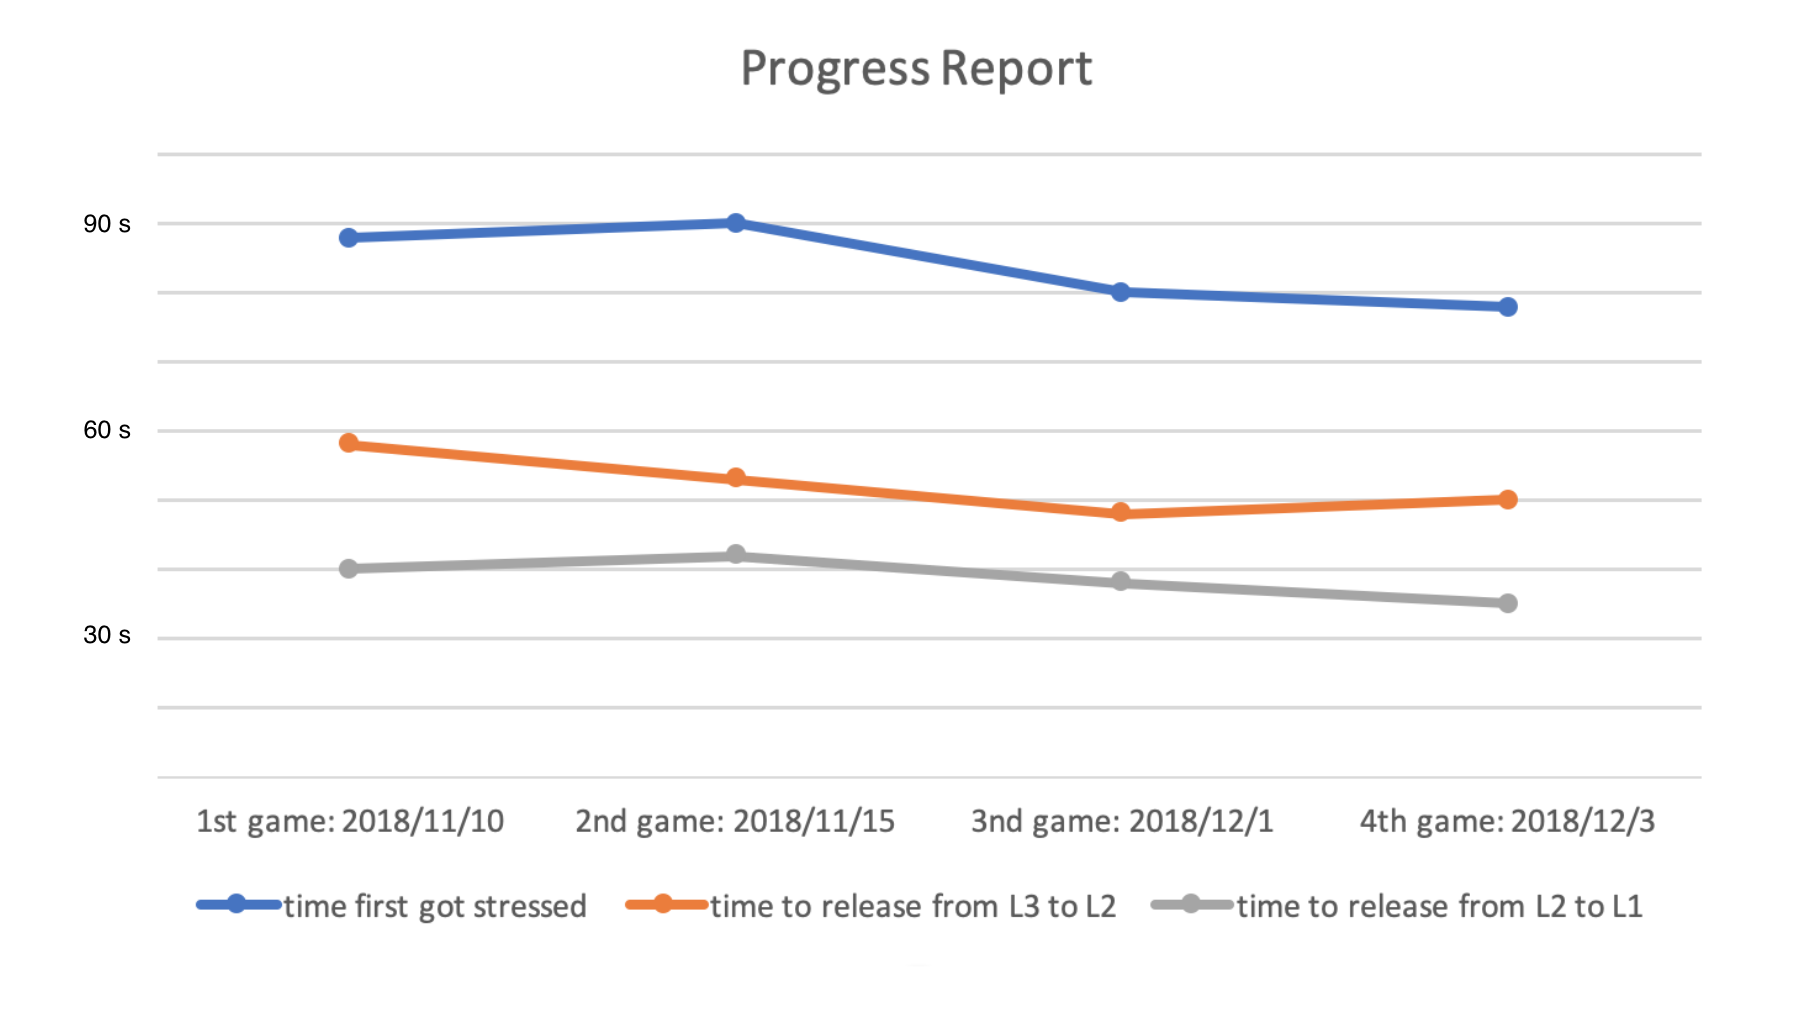
\includegraphics[width=0.75\linewidth]{progress-report.png}
    \caption{Progress Report}
    \label{fig:prog-rep}
\end{figure} 











\chapter{Technologies Used} % Jake
\chapter{Architectural Diagram} % Brendan

% Event-driven architecture

Figure 7.1 shows the event-driven architecture our system uses. When a change of state occurs in a model, it broadcasts an event to everything around it.
\begin{figure}[ht]
    \centering
    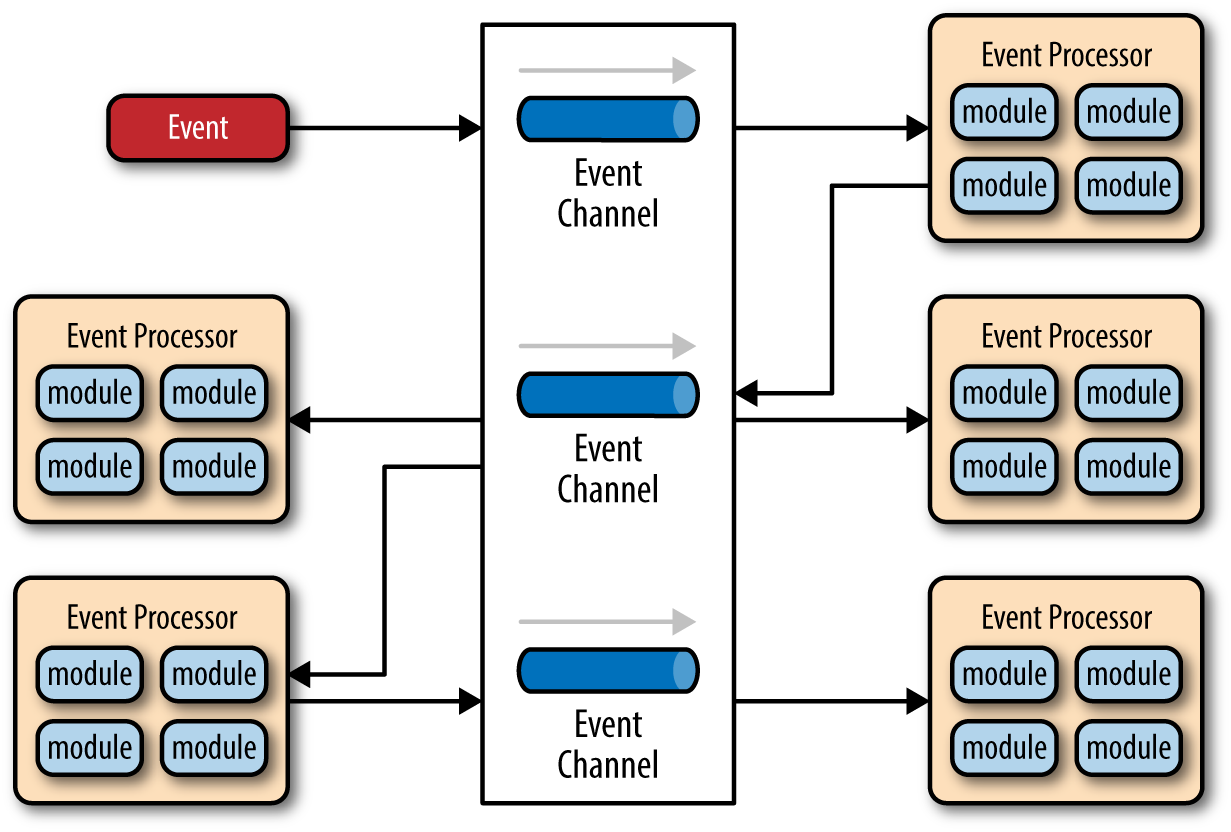
\includegraphics[scale=1.5]{eventarchitecture.png}
    \caption{Event-Driven Architecture}
\end{figure}
\chapter{Design Rationale}

\section{Virtual Reality}
    A virtual reality interface was chosen due to the immersive experience it provides. Users of the system are practicing for real-life situations, and in order to get the most out of the experience, the system must be as close to real life as possible. Virtual reality provides the closest experience to reality, without any keyboard controls to interface through. Moving through a virtual environment provides valuable experience for reacting to the real-life situations this program hopes to train people in.
\section{Google Cardboard}
    Google Cardboard technology was chosen due to the low cost of usage, providing a more cost-effective solution to virtual reality hardware than many of the major competitors, while still giving a quality experience. By offloading the software requirements to a smartphone and keeping the hardware down to a cardboard frame, Google Cardboard lets the product scale more effectively among users and increases accessibility.
\section{Biofeedback}

\section{Event-Based Architecture}
\chapter{Test Plan} \label{test-plan} % Jake [DONE]
% see 101718.pdf in COEN 174 notes
Testing is fundamental for ensuring that our product works effectively for its users. Throughout this project, we will utilize testing to verify our product works and validate that we were building the right product. 

\section{White Box Testing}

As we develop this project, we will be constantly testing and debugging our solution. Since we are using GitHub for reasons mentioned in Section~\ref{tech-used}, this will simplify deploying our system and verifying if changes are functioning correctly.

\subsection{Unit Testing}
    We will divide our functionality into modules to implement unit testing. We will create a testing directory that includes test cases for each of these respective modules.
\subsection{Integration Testing}
    After unit testing is complete, we will incorporate multiple modules to test together. We will test to verify our navigation functionality, allowing for a more seamless experience for black box testers.
\section{Black Box Testing}

Prior to beginning black box testing, we will need to receive permission from the SCU Institutional Review Board to conduct research with human participants.
% https://www.scu.edu/provost/research/research-compliance-and-integrity/human-subjects/
\subsection{System Testing}
    We will enlist testers to test the integrated system to evaluate the system’s compliance with our specified requirements. They will test our mobile application on different hardware to ensure portability.
\subsection{Acceptance Testing}
    For our final phase of testing, we will test with parents enrolled in Dr. Burn's Resilient Families Program.
\chapter{Risk Analysis} % Jake [DONE]

\section{Risk Analysis Table}

Our team identified the most common and severe risks during the software development process. Table \ref{table:risk-anal} presents these risks, along with their potential consequences and solutions. The impact of each risk results from the product of their respective probability and severity. The risks are listed from highest to lowest impact.   

\begin{table}[h!]
\centering
\caption{Risk Analysis}
\label{table:risk-anal}
\vspace{5mm}
\resizebox{\textwidth}{!}{%
\begin{tabular}{@{}llllll@{}}
\toprule
\textbf{Name of Risk} &
    \textbf{Consequences} &
    \textbf{Probability} &
    \textbf{Severity (0-10)} &
    \textbf{Impact} &
    \textbf{Mitigation Strategies} \\
    \midrule
    Bugs &
    \makecell[l]{Must allocate time \\
        dedicated to debugging } &
    1.0 &
    2 &
    2.0 &
    \makecell[l]{Maintain thorough documentation of code \\        Perform rigorous unit testing} \\
    \midrule
    \makecell[l]{Misunderstood \\ 
        requirements } &
    \makecell[l]{System requirements \\
        are not met } &
    0.2 &
    9 &
    1.8 &
    \makecell[l]{Perform code reviews \\ 
        Frequent, effective communication \\ 
        Allow users to provide feedback } \\
    \midrule
    \makecell[l]{Technical \\
        limitations } &
    \makecell[l]{Unable to implement \\
        certain requirements } &
    0.5 &
    3 &
    1.5 &
    \makecell[l]{Familiarize ourselves with technologies used \\
        Be honest regarding technical skills} \\
    \midrule
    \makecell[l]{Compatibility \\
        issues } &
    \makecell[l]{Components do not \\ 
        function together properly } &
    0.3 &
    4 &
    1.2 &
    \makecell[l]{Modularize code (loose coupling, high cohesion) \\
        Use git as version control system to track changes} \\
    \midrule
    Time & 
    \makecell[l]{System not complete \\
        by deadline } & 
    0.1 &
    8 &
    0.8 &
    \makecell[l]{Follow development timeline \\ 
        Schedule weekly team meetings \\ 
        Re-evaluate necessity of features} \\
    \bottomrule
\end{tabular}%
}
\end{table}
\chapter{Development Timeline}

\backmatter
\end{document}
